%!TEX ROOT=../ctutest.tex

\chapter{Introduction}
\label{chap:intro}

My dissertation, as well my long-term research, centers around the field of \textit{automated fact checking} through the means of Natural Language Processing (NLP) and its modern methods.
The work consists of the analysis of the whole fact-checking process, its subdivision and simplification into tasks that can be efficiently addressed using the current state-of-the-art NLP methods, collection of data appropriate to benchmark such tasks, delivery of example solutions and their validation against similar research in other languages and related tasks.

The main focus of mine and of our research group are the fact-checking-related tasks in the West Slavic languages (Czech, Slovak and Polish) and secondarily in English.
My contribution has so far been the collection and publication of novel datasets for the fact-checking task and its subroutines, models trained for the tasks and their debate, including the ongoing establishment of metrics that would explainably rate the model success and error rates in terms close to the human notion of \textit{facticity} (which proves to be a challenge on its own, requiring another round of novel research~\cite{ffci,wright}). 

My doctoral aim is to cover every step on the path from gathering a factual claim -- for example, extracting it from a political debate -- to predicting its veracity verdict and justifying it rigorously with hard data.
With the recent boom in NLP beginning with the advent of transformer networks and later the Large Language Models (LLMs)~\cite{llms}, few-shot learning~\cite{gpt3} and prompting~\cite{prompting} a significant part of the research is and has to be an appropriate and timely adoption of new ever-evolving sota NLP solutions, based on well-designed studies in our specific context.

Overall, my agenda is to follow up on my published research on fact checking in Czech with methods that reiterate on our results in other languages and evolving our previous methodology based on transformer \textit{pre-training \& fine-tuning} paradigm to a computationally feasible design based on LLMs, which are already exhibiting superiority tasks similar to ours~\cite{bing} in English.

My recent focus within the whole grand fact-checking scheme is the step of \textit{claim generation}, which I aim to establish among the other commonly benchmarked NLP tasks within the scientific community, adjacent to that of \textit{abstractive summarization}.
To benchmark the task, one would need a set of metrics that properly reflect phenomena such as \textit{model hallucinations} -- a common problem of modern day LLMs~\cite{Ji_2023}.
As the exact word-level metrics for NLP generative tasks do not correlate well with human judgement~\cite{bert-score} and model-based metrics are hard to explain, my research also focuses on a delivery of a set of human-understandable model-based metrics.

The goal of this study is to show the directions I am taking to address these challenges, reasoning behind them, my research questions and current results that motivated them.

\section{Motivation}
\label{sec:motivation}

\begin{figure}
    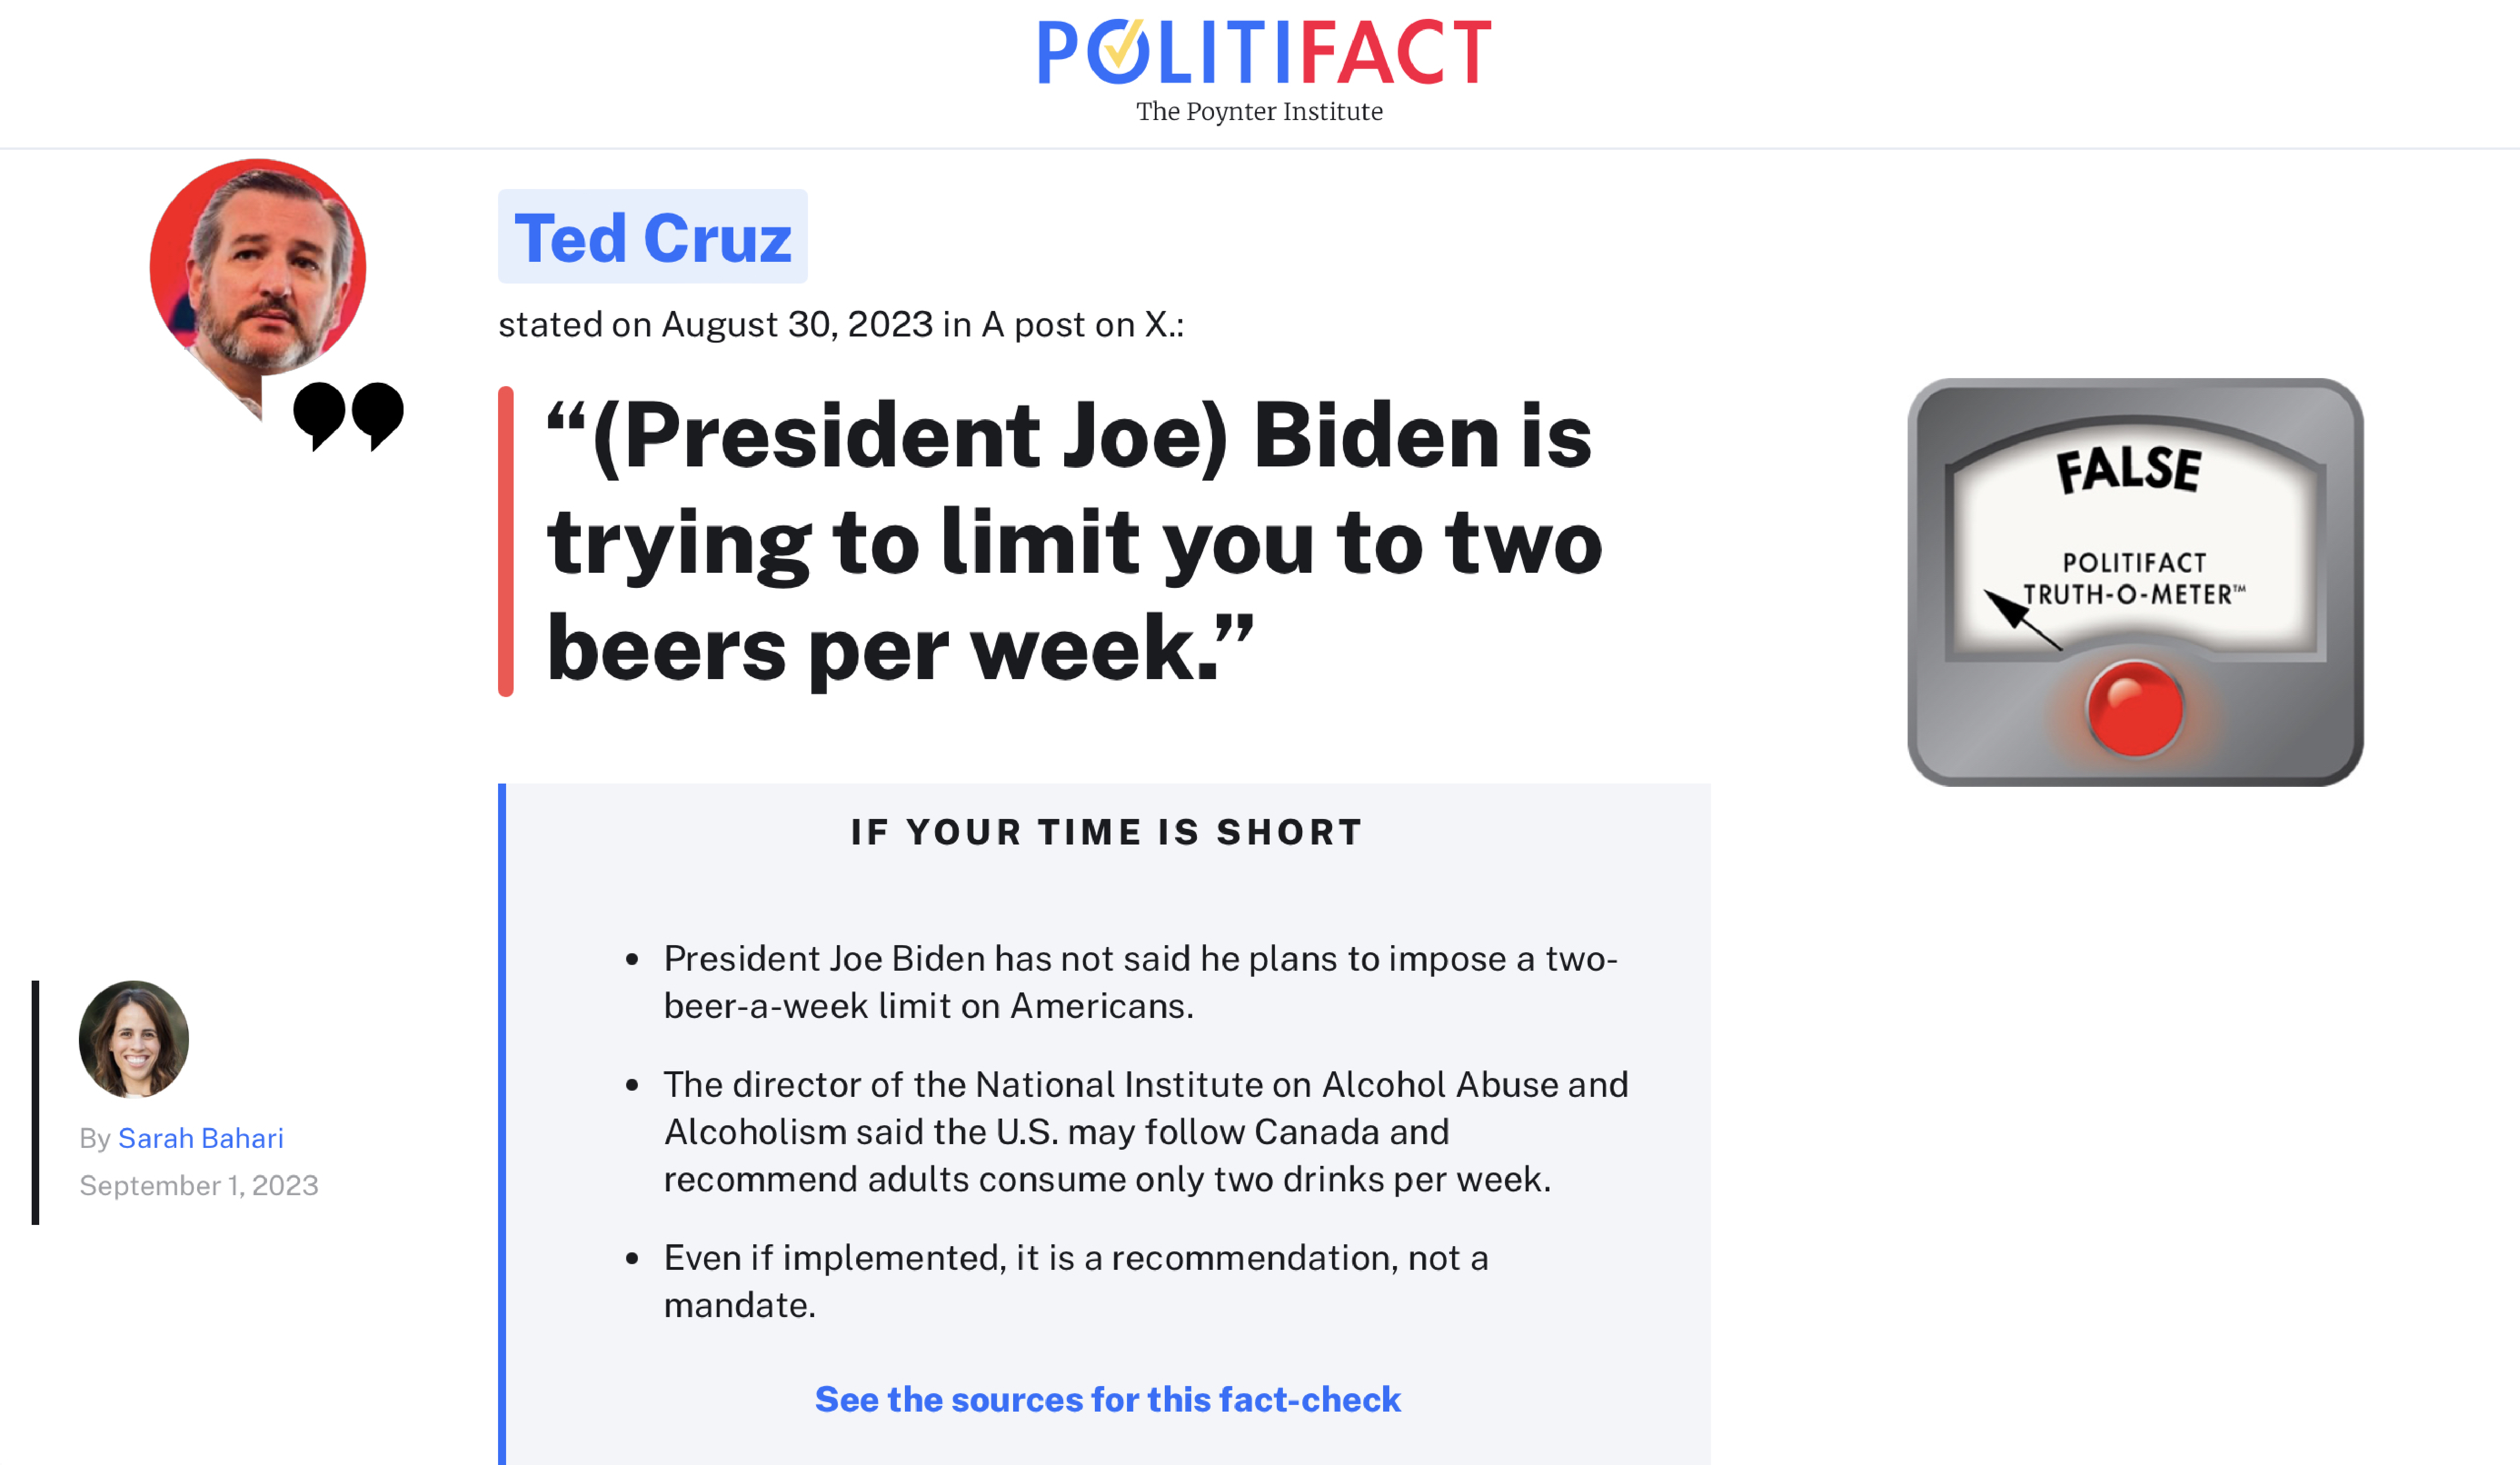
\includegraphics[width=14cm]{fig/politifact.pdf}
    \caption{A real world example of fact checking done by \url{https://politifact.org}}
    \label{fig:politifact}
\end{figure}

The spread of misinformation in the online space has a growing influence on the Czech public~\cite{stem}. It has been shown to influence people's behaviour on the social networks~\cite{Lazer1094} as well as their decisions in elections~\cite{10.1257/jep.31.2.211}, and real-world reasoning, which has shown increasingly harmful during the COVID-19 pandemic~\cite{BARUA2020100119} and the Russo-Ukrainian war~\cite{georgiana_stanescu_2022_6795674}.

The recent advances in artificial intelligence have unintentedly contributed to the spread of misinformation on social media~\cite{doi:10.1177/2056305119888654}, as well as they hold a large potential for the false content generation~\cite{glorin}.

Recent research has shown promising results~\cite{fever2} in false claim detection for data in English, using a trusted knowledge base of true claims (for research purposes typically fixed to the corpus of \textsf{Wikipedia} articles), mimicking the \textit{fact-checking} efforts in journalism.

Fact-checking (Figure~\ref{fig:politifact}) is a process of matching every information within a \textit{factual claim} to its \textit{evidence} (or \textit{disproof}) in trusted data sources to infer the claim veracity and verifiability. In exchange, if the trusted \textit{knowledge base} contains a set of \"{ground truths} sufficient to fully infer the original claim or its negation, the claim is labelled as {\techbf{supported}} or {\techbf{refuted}}, respectively. If no such \textit{evidence set} can be found, the claim is marked as {\techbf{unverifiable}}\footnote{Hereinafter labelled as \texttt{NOT ENOUGH INFO}, in accordance to related research.}.


\section{Automated Fact Checking}

\begin{figure}
    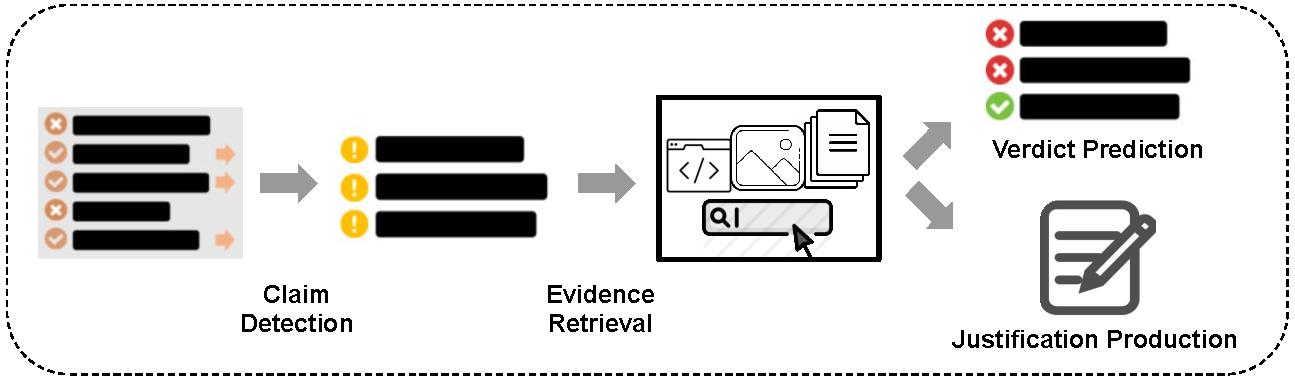
\includegraphics[width=14cm]{fig/framework.pdf}
    \caption{Automated fact-checking pipeline, reprinted from~\cite{guo-etal-2022-survey}}
    \label{fig:framework}
\end{figure}

Despite the existence of end-to-end fact-checking services, such as \url{politifact.org} or \url{demagog.cz}, the human-powered approach shows weaknesses in its scalability. By design, the process of finding an exhaustive set of evidence that decides the claim veracity is much slower than that of generating false or misguiding claims. Therefore, efforts have been made to move part of the load to a computer program that can run without supervision.

The common research goal is a fact verification tool that would, given a claim, semantically search provided knowledge base (stored for example as a \textit{corpus} of some natural language), propose a set of evidence (e. g. $k$ semantically nearest paragraphs of the corpus) and suggest the final verdict (Figure \ref{fig:framework})~\cite{guo-etal-2022-survey}. This would reduce the fact-checker's workload to mere adjustments of the proposed result and correction of mistakes on the computer side. 

The goals of the ongoing efforts of {\textsf{FactCheck}} team at {\textsf{AIC CTU}}, are to explore and adapt the state-of-the-art methods used for fact verification or similar tasks in other languages, currate appropriate datasets for it and propose strong systems for such a task in Czech.


\section{A word on the Transformers}
\label{sec:transformers}
For the past six years, the state-of-the-art solution for nearly every Natural Language Processing task is based on the concept of \textit{transformer networks} or, simply, \textit{Transformers}. This has been a major breakthrough in the field by~\cite{vaswani}, giving birth to the famous models such as \textsf{Google}'s \textsf{BERT} encoder~\cite{bert} and its descendants, or the \textsf{OpenAI}'s \textsf{GPT-3} decoder~\cite{gpt3} and \textsf{GPT-4}~\cite{gpt4} that are used in the booming online AI service \textsf{ChatGPT}\footnote{\url{https://chat.openai.com}}.

In our proposed methods, we use Transformers in every step of the fact verification pipeline. Therefore, we would like to introduce this concept to our reader to begin with. 

Transformer is a neural model for \textit{sequence-to-sequence} tasks, which, similarly e.g. to the \textit{LSTM-Networks}~\cite{lstm}, uses the Encoder--Decoder architecture. Its main point is that of using solely the \textit{self-attention} mechanism to represent its input and output, instead of any sequence-aligned recurrence~\cite{vaswani}.

In essence, the \textit{self-attention} (also known as the \textit{intra-attention}) transforms every input vector to a weighted sum of the vectors in its neighbourhood, weighted by their \textit{relatedness} to the input. One could illustrate this on the \textit{euphony} in music, where every tone of a song relates to all of the precedent and successive ones, to some more than to the others.

The full Transformer architecture is depicted in Figure~\ref{fig:transformer}.

\begin{figure}
    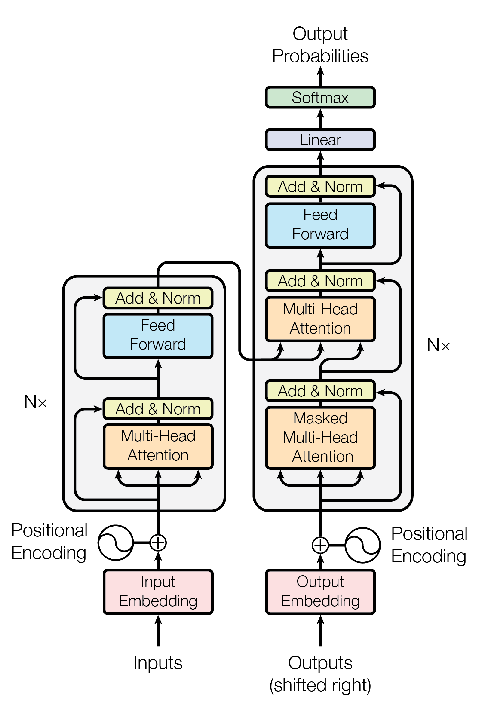
\includegraphics[width=9cm]{fig/transformer.pdf}
    \caption{Transformer model architecture, reprinted from~\cite{vaswani}}
    \label{fig:transformer}
    \end{figure}
    %--- /FIG

\section{Dissertation minimum study outline}
 
\begin{itemize}
\item {\techbf{Chapter~\ref{chap:intro}}} introduces the dissertation topic, motivates the research sets up our challenges for the future research 

\item {\techbf{Chapter~\ref{chap:sota}}} examines the most relevant research in the field and tries to highlight the recent paradigm shift from models trained for a single task to a single large models that perform well in everything

\item {\techbf{Chapter~\ref{chap:contribution}}} explains our current contributions to the field of automated fact-checking and NLP in Czech

\item {\techbf{Chapter~\ref{chap:plan}}} describes our plan for the dissertation and justifies the directions we are taking

\item Finally, {\techbf{Chapter~\ref{chap:conclusion}}} concludes the study with a wrapup of its findings

\end{itemize}

